\documentclass{article}
\include{graphicx}
\begin{document}
\title{Supplement to ``Rapid, accurate peptide identification''}

\author{Chris Y. Park, Aaron A. Klammer, Lukas K\"{a}ll, Michael J. MacCoss
and William S. Noble}

\maketitle

\begin{figure}
  \centering
  \begin{tabular}{ll}
    {\sf A} & {\sf B} \\
    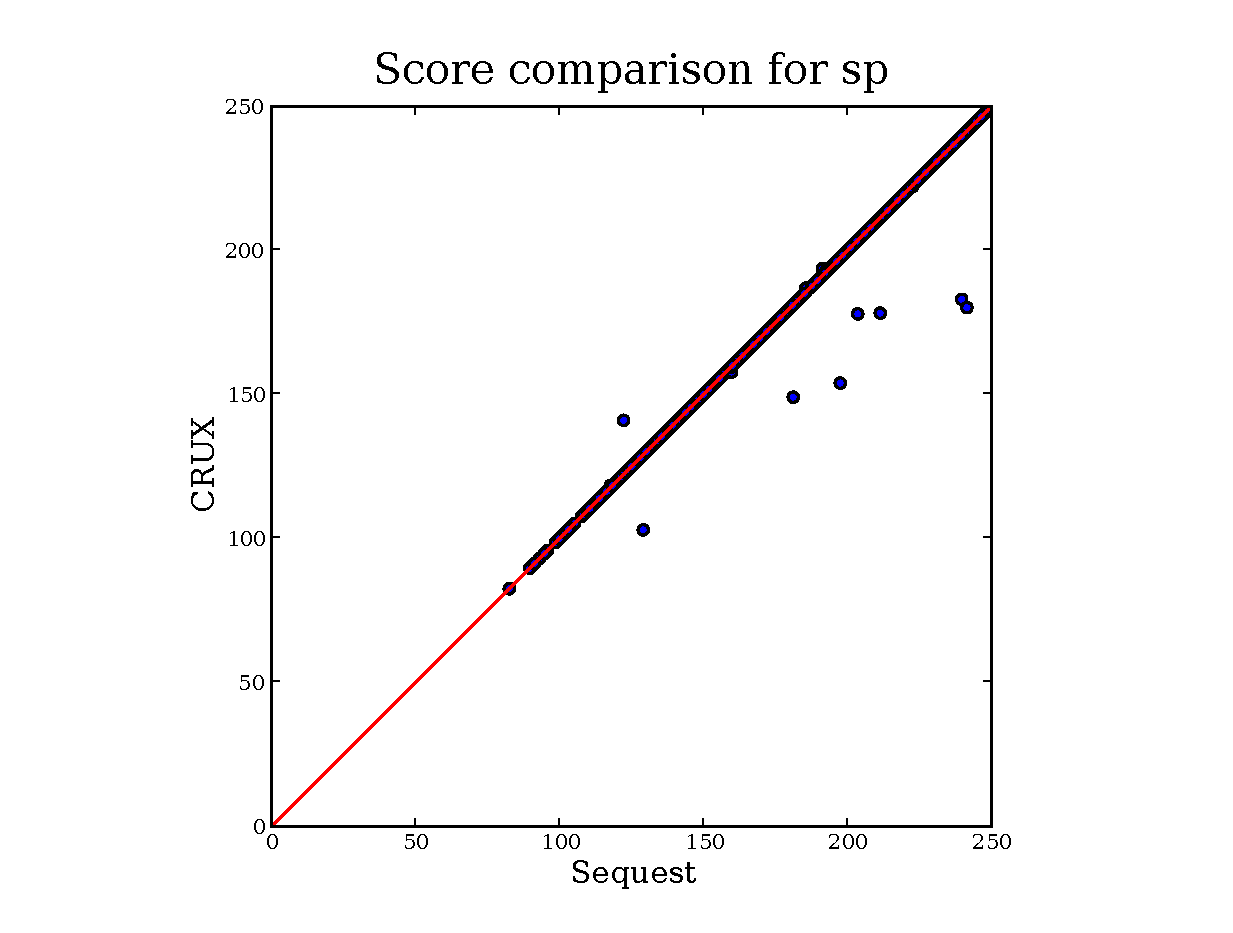
\includegraphics[width=2.5in]{../../results/paper-figure/second-score/fig-2-random-sp.eps} &
    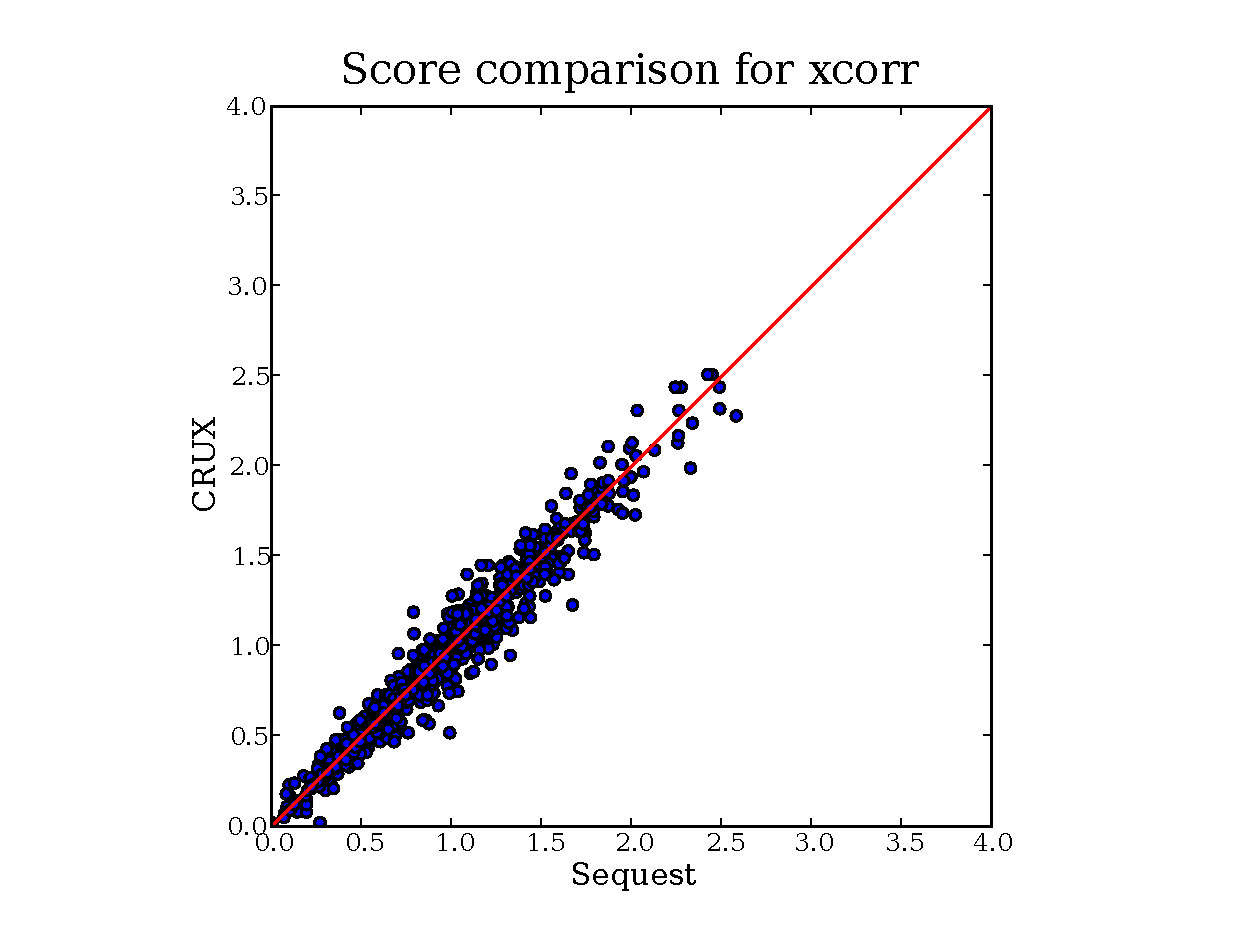
\includegraphics[width=2.5in]{../../results/paper-figure/second-score/fig-2-random-xcorr.eps} \\
  \end{tabular}
  \caption{{\bf Re-implementation of $Sp$ and $Xcorr$ scoring functions.}
  The figure plots, for a collection of randomly generated spectra and
  randomly associated peptides 
  $Sp$ ({\sf A}) and $XCorr$ ({\sf B}) scores as computed by Crux as a function of the
  same scores as computed by {\sc Sequest}. 
  \label{figure:sp-xcorr-random}}
\end{figure}

\begin{figure}
  \centering
  \begin{tabular}{ll}
    {\sf A} & {\sf B} \\
  \includegraphics[width=2.5in]{../../results/paper-figure/index/indexing-yeast.eps} &
  \includegraphics[width=2.5in]{../../results/paper-figure/turbo-no-missed/indexing-yeast-windows.eps} \\

\end{tabular}
  \caption{{\bf Rapid retrieval of candidate peptides.}  The figure
  plots the total running time required to search 100 tandem mass
  spectra against the yeast protein databases
  on computers running the Linux ({\sf A}) 
  or Windows ({\sf B}) operating systems, using {\sc Sequest} and Crux with 
  and without indices.
  Run time is plotted 
  as a function of the mass tolerance used to define candidate
  peptides. The Linux OS plots have three series
  because indexed {\sc Sequest} searches with are only possible on Windows.
  \label{figure:indexing}}
\end{figure}


\end{document}
